% -*- root: ../thesis.tex -*-
%!TEX root = ../thesis.tex
% ******************************* Thesis Chapter 2 ****************************


% ----------------------- paths to graphics ------------------------

% change according to folder and file names
\graphicspath{{2_background/figures/}}
% ----------------------- contents from here ------------------------

To fully comprehend the papers to be presented, we present a general overview of the needed concepts.
A short introduction to the basic theory of \acl{GPs} as well as their extension to large datasets using inducing points \cite{Titsias2009} is given in Chapters~\ref{ch:classification},~\ref{ch:multiclass} and \ref{ch:general}, however a more thorough and basic description is given in this chapter.
Additionally, this chapter dives more into the basics of probabilistic Bayesian modeling, variational inference, and sampling methods.

\section{Probabilistic Bayesian Modeling}

\label{sec:prob_bayes}

Bayes' theorem is one of the simplest theorems in probability theory, and its proof fits in one line, yet its implications are unmeasurably important.

Let us give a very general modeling setting that we will follow for the rest of this chapter.
Given a set of observed variables $\bX$, a set of latent (unobserved) variables $\btheta$ with a \textbf{prior} distribution $p(\btheta)$, and a \textbf{likelihood} function $p(\bX|\btheta)$, we obtain the \textbf{posterior} distribution $p(\btheta|\bX)$ via Bayes' theorem:
\begin{align}
p(\btheta|\bX) = \frac{p(\bX|\btheta)p(\btheta)}{p(\bX)} = \frac{p(\bX|\btheta)p(\btheta)}{\int p(\bX|\btheta)p(\btheta)d\btheta}.
\label{eq:bayes}
\end{align}

Here $p(\bD)$ represents the so-called evidence and can be used to compare different models (the dependency on the used model is implicit here).
The posterior allows us to obtain a distribution of the latent variables with its uncertainty given the prior $p(\btheta)$ and the data $\bX$.
The posterior is used for computing all kinds of expectations of the form $\expec{p(\btheta|\bX)}{f(\btheta)} = \int f(\btheta)p(\btheta|\bX)d\btheta$.
Expected values of interest can be statistics of the posterior like the mean ($\expec{p(\btheta|\bX)}{\btheta}$) or predictive distribution of new data points $p(\bx'|\bX) = \expec{p(\btheta|\bX)}{p(\bx'|\btheta)}$.

Let's take the simple example of linear logistic regression, a discriminative model:
Given an input $\bx \in \mathbb{R}^D$ and a binary label $y\in \{ 0, 1\}$, we model the process as:
\begin{align}
    y \sim \Be\left(\sigma(\btheta^\top \bx)\right),
\end{align}
where $\Be$ is the Bernoulli distribution, $\btheta\in\mathbb{R}^D$ is a vector of weights (our latent variable), and $\sigma$ is the logistic function $\sigma(x) = \frac{1}{1 + \exp(-x)}$, i.e. $\sigma : \mathbb{R} \mapsto [0, 1]$.
The likelihood function is given by: $p(y_i|\btheta,\bx_i) =\sigma\left(\btheta^\top \bx_i\right)^{y_i}\sigma\left(-\btheta^\top \bx_i\right)^{1-y_i}$ for an output label $y_i$ and input features $\bx_i$.

Now let's suppose that we have $N$ pairs of input $\bx_i$ and label $y_i$, that we assume to be \ac{iid}, we get a training set $\bX = \{\bx_1,\ldots,\bx_N\}$, $\boldy = \{y_1,\ldots,y_N\}$.
With a prior distribution $p(\btheta)$ on $\btheta$, we build the posterior as $p(\btheta|\boldy,\bX) \propto p(\btheta)\prod_{i=1}^N p(y_i|\btheta, \bx_i)$.
Predictions for a new data input $\bx^*$ can be then computed as:
\begin{align}
p(y^*|\bx^*,\boldy,\bX) = \int p(y^*, \btheta|\bx^*\boldy, \bX)d\btheta = \int p(y^*|\btheta,\bx^*) p(\btheta|\boldy,\bX)d\btheta.
\end{align}

Note that the last term of the equation directly involves the posterior distribution $p(\btheta|\by,\bX)$.
To solve this integral, we must either know the posterior distribution and compute the integral numerically (or analytically) or sample from the posterior and estimate the integral using Monte-Carlo integration

\subsection{Posterior computations}
\label{sec:posterior}
Given a prior $p(\btheta)$ and a likelihood $p(\bx|\btheta)$, computing the posterior \eqref{eq:bayes} in closed-form requires the integral $p(\bx)=\int p(\bx|\btheta)p(\btheta)d\btheta$.
\com{the integral is not enough}
For most non-trivial models, this integral is intractable, and approximations to the posterior are needed.
Such methods are introduced in Section~\ref{sec:approx_inf}.
However, in specific settings, computing the posterior in closed-form is possible.
When the prior is said \textbf{conjugate} to the likelihood, the posterior is of the same probability distribution family as the prior and can be computed analytically \cite{schlaifer1961applied}.
It is worth emphasizing this seemingly trivial case since it will be exploited in Section~\ref{sec:scale-mixtures}.
For a general example, we consider a likelihood part of the \textbf{exponential family}:
\begin{align}
    p(\bx|\btheta) = h(\bx)\exp(\boldeta(\btheta)^\top T(\bx) - A(\btheta)),
    \label{eq:explikelihood}
\end{align}
where $\btheta$ are the \textbf{distribution parameters}, $h(\bx)$ is the \textbf{base measure}, $\boldeta(\btheta)$ corresponds to the \textbf{natural parameters}, $T(\bx)$ is the \textbf{sufficient statistics} and $A(\btheta)$ is the \textbf{log-partition}.

Formally, a \textbf{conjugate prior} to the likelihood \eqref{eq:explikelihood} is defined as:
\begin{align}
    p(\btheta|\balpha) = h'(\btheta)\exp(\boldeta'(\balpha)^\top T'(\btheta) - A'(\balpha)),
    \label{eq:expprior}
\end{align}
where $T'(\btheta) = \left\{\boldeta(\btheta), A(\btheta)\right\}$ and where $\balpha$ is the prior distribution parameters.
Given a factorizable likelihood $p(\bX|\btheta) = \prod_{i=1}^N p(\bx_i|\btheta)$, the posterior will be proportional to
\begin{align}
    p(\btheta|\bX) \propto h'(\btheta)\exp\left(\left(\{\sum_{i=1}^N T(\bx_i), N\} + \boldeta'(\balpha)\right)^\top T'(\btheta)\right).\label{eq:posterior}
\end{align}
Note that the only dependence on $\bX$ is via the sufficient statistics $T(\bx)$.

Conjugate models are very practical as the posterior can be found in one step, but due to the constraints also tend to be too simple for complex real-world models.

If the prior is not conjugate of the likelihood, an alternative is to look for \textbf{conditionally conjugacy}.
A parameter $\theta_i$ with a conditionally conjugate prior will have a full-conditional distribution of the same family.
The full-conditional distribution is defined as $p(\theta_i|
\bX, \btheta_{/i})$ where $\btheta_{/i} = \{\theta_1, \ldots, \theta_{i-1},\theta_{i+1},\ldots\theta_D\}$.
This notion of full-conditional also extends to blocks of variables.
If we translate our exponential family example from above, we look for In the same exponential family example in equation \eqref{eq:expprior}, we are interested in the conjugate prior to the distribution $p(\bX, \btheta_{/i} | \theta_i)$

\section{Gaussian Processes}
\label{sec:gps}

\acf{GPs} are a class of stochastic processes used as non-parametric probabilistic representations to functions.
A \ac{GP} is a stochastic process $\{f_t;t\in T\}$, where the joint distribution on any finite collection of random variables $\{f_t\}$ follows a (multivariate) Gaussian distribution \cite{rasmussen2006gaussian}.
Linear operations on Gaussian variables can be done analytically, which makes them computationally very attractive.
For instance, marginals can be computed exactly, and a product of Gaussian distributions of the same variable is still proportional to another Gaussian.
% The Gaussian distribution is to statistics what the harmonic oscillator is to physics".

A \ac{GP} is uniquely specified by its \textbf{mean function} $\mu_0(\bx)$ and \textbf{kernel function} (also called covariance function) $k(\bx, \bx')$.
$\mu_0(\bx)$ can be any real-valued function while $k(\bx, \bx')$ needs to be a positive-definite function (also called Mercer kernels).
A symmetric function $k:\mathcal{X}\times\mathcal{X}\rightarrow \mathbb{R} $ is positive-definite on $\mathcal{X}$ if $\boldsymbol{w}^\top K \boldsymbol{w}$ where $K_{ij} = K(\bx_i,\bx_j)$ for any $\boldsymbol{w}\in\mathbb{R}^N$ and any $\{\bx_i,\ldots,\bx_N\} \in \mathcal{X}$.

One of the interpretations of a \ac{GP}($\mu_0$, $k$) is as a prior on the function space.
To perform concrete computations, we need to project it into a finite-dimensional space.
Given a random function $f$ we wish to represent with a \ac{GP}, we can project $f$ into a finite space by evaluating it on a set of data inputs $\bX = \{\bx_1, \ldots, \bx_N\}$ such that we obtain the finite-dimensional vector $\boldf$ where $f_i = f(\bx_i)$.
The prior on the projected \ac{GP} on $\bX$ is given by $\mathcal{N}\left(\bmu_0(\bX), K_{X}\right)$ where $\bmu_0(\bX) = \{\mu_0(\bx_i)\}_{i=1}^N$ and $K \in \mathbb{R}^{N\times N}$ is the kernel matrix, defined by $K_{ij} = k(\bx_i, \bx_j)$.

\subsection{Gaussian Process Regression}

Let us have a look at the most standard problem: Gaussian regression.
Given our prior $p(\boldf) = \No(\boldf|\bmu_0, \bK)$, we can add noisy observations $\by = \{y_i\}_{i=1}^N$ for each respective $\bx_i$ and model the process as:
\begin{align}
y_i = f(\bx_i) + \epsilon_i,
\end{align}
where $\epsilon_i \sim \No(0,\sigma^2)$.
This leads to the likelihood $p(y_i|f_i) = \No(y_i|f_i, \sigma^2)$.
Fortunately, adding a zero-mean Gaussian variable to another leads to another Gaussian distribution function with increased variance and the posterior for $\boldf$ is given by $p(\boldf|\by) = \No(\boldf|\by, \bK + \sigma^2 I)$.
The predictive distribution of $f_*=f(\bx_*)$ on a new input $\bx_*$ can be evaluated by computing:
\begin{align}
p(f_*|\bx_*,\bX,\by) = \int p(f_*|\boldf,\bx_*)p(\boldf|\bX,\by)d\boldf.
\end{align}	
This integral is analytically tractable and results in 
\begin{align}
    p(f_*|\bx_*,\bX,\by)=\No(f_*|m_*,s_*),
    \label{eq:pred_gp}
\end{align}
where $m_* = K_{\bx_*,\bX}(K_{\bX,\bX} + \sigma^{2}I)^{-1}\boldy$ and $s_*=K_{\bx_*,\bx_*} - K_{\bx_*,\bX}\left(K_{\bX,\bX}+\sigma^2I\right)^{-1}K_{\bX,\bx_*}$.
The predictive distribution for $f_*$ is Gaussian, with a known mean $m_*$ and a measure of uncertainty given by the variance $s_*$.
Note that $s_*$ depends directly on $K_{\bx_*,\bX}$: if $\bx_*$ is far from all points in $\bX$ (in the sense of the distance used in the kernel $k$), then $K_{\bx_*,\bX}$ will be very small and the variance $s_*$ maximized.
When new inputs $\bx_*$ are distant from the training data $\bX$, the predictive uncertainty will be high.\com{to come back to clarify}
A concrete example is shown on Figure~\ref{fig:gp_example}.

\begin{figure}
    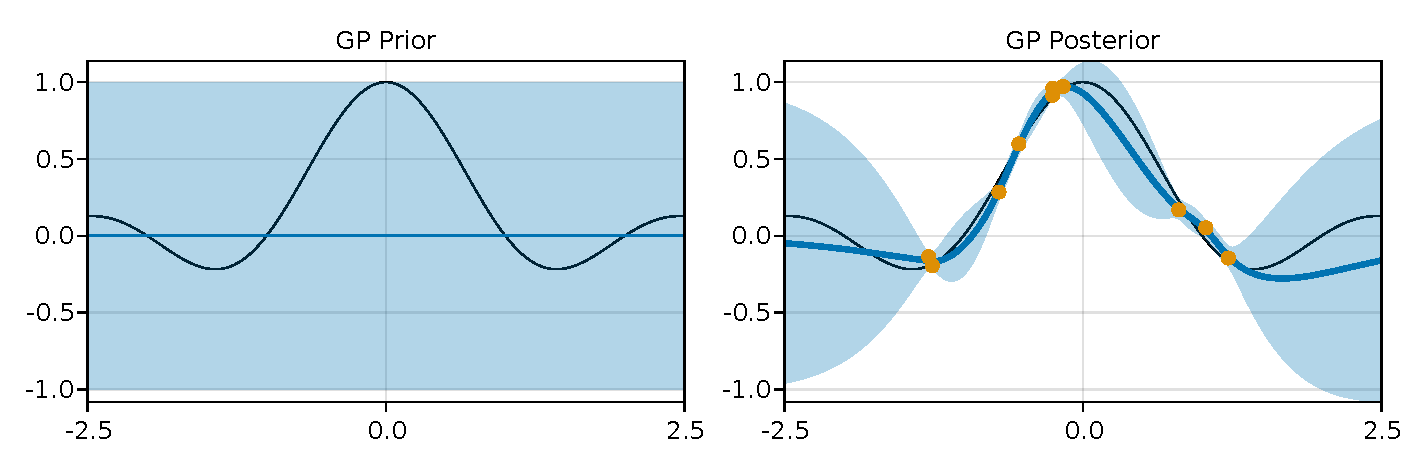
\includegraphics[width=\textwidth]{./chapters/2_background/figures/GP_example.pdf}
    \caption{Illustration of the realization of a Gaussian Process. The black is the true function $f$, the blue line is the mean of the prediction, the blue area represent the confidence interval of 2 standard deviations, the orange points represent observed data. Left: prediction on a grid given no observations. Right: prediction on a grid given a set of observations}
    \label{fig:gp_example}
\end{figure}

\subsection{Non-Conjugate Gaussian Processes}
\label{sec:nonconj_gps}
A Gaussian prior is only conjugate to the mean parameter of a Gaussian likelihood.
Therefore, the \ac{GP} posterior obtained in the previous section is only tractable for homoscedastic (the noise variance is independent of the input) Gaussian likelihoods, for all other cases we talk about \textbf{non-conjugate \ac{GPs}}.
Examples of non-conjugate \ac{GPs} problems are binary classification, regression using non-Gaussian noise such as Student-t or Laplace noise, or Poisson regression.
Other examples, such as multi-class classification or heteroscedastic regression, require multiple latent \ac{GPs}.
Figure~\ref{fig:gp_class_example} shows an example of 1-dimension binary classification with a \ac{GP} where the posterior was approximated using variational inference (see Section~\ref{sec:vi}).
Although the \ac{GP} does not recover exactly the true process, it is confidently in its interval.

Posteriors of non-conjugate problems are not analytically tractable, and one needs to resort to the approximation methods presented in Section~\ref{sec:approx_inf}.
A strong focus of this thesis is to take these non-conjugate likelihoods and find a representation where inference is simplified and basic methods can be used.

\begin{figure}
    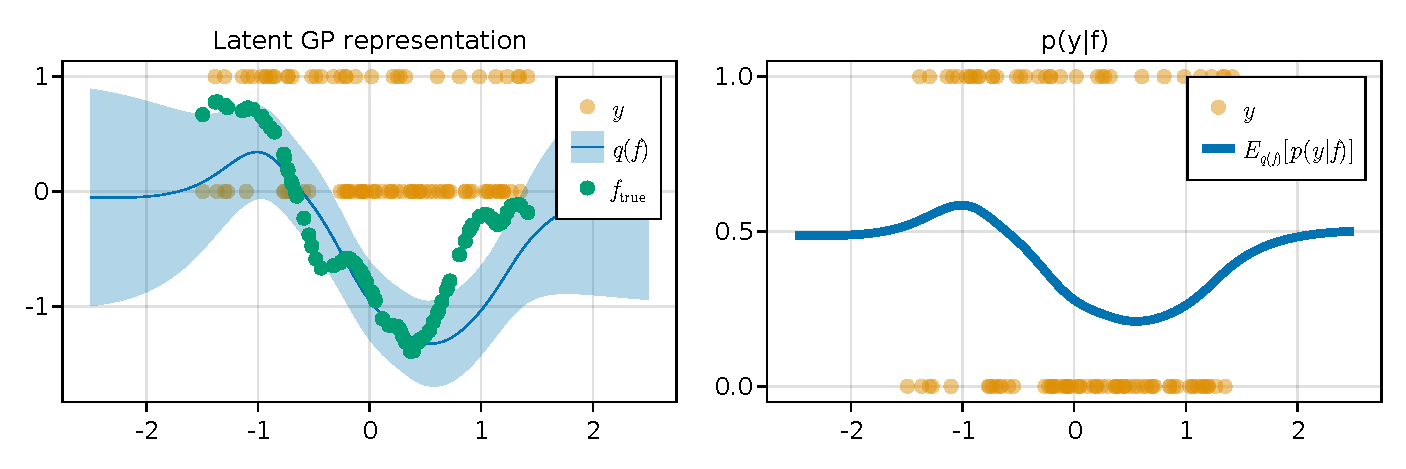
\includegraphics[width=\textwidth]{./chapters/2_background/figures/GP_classification_example.pdf}
    \caption{Illustration of a latent Gaussian process used for a binary classification problem.
    The Bernoulli likelihood is linked to the latent \ac{GP} via the logistic function.
    On the left is shown the optimal variational posterior $q(f)$ in blue, compared to the true generation of $f$ in green.
    Similar to Figure~\ref{fig:gp_example}, the blue band represents one standard deviation.
    On the right, we show the expected predictive probability for $y$ given the variational posterior $q(f)$ in blue.}
    \label{fig:gp_class_example}
\end{figure}

\subsection{Sparse Gaussian Processes}
\label{sec:sparsegps}
One of the other largest drawbacks of \ac{GPs}, regardless of the conjugacy of the likelihood, is the scalability with the number of observed samples.
When computing the predictive mean and covariance, the inverse matrix operation in Equation~\ref{eq:pred_gp} has a computational complexity of $\mathcal{O}(N^3)$ where $N$ is the number of samples.
For one-dimensional inputs ($D=1$), solutions exist for specific kernels using state-space models representation \cite{pmlr-v9-turner10a,solinInfiniteHorizonGaussianProcesses2018}, leading to an $\mathcal{O}(N)$ complexity but higher-dimensional problems require alternative solutions.
The first approach to reduce the complexity was to use a Nystr\"om approximation \cite{williams2002observations}.
\citet{csato2002sparse} proposed to create an approximation of the posterior using a subset of the points only in the context of online learning.
\citet{snelsonSparseGaussianProcesses2009} expanded this theory to the offline framework and \citet{csato2002gaussian} followed by \citet{Titsias2009} developed an alternative approximation based on KL divergence where the "inducing points" are not necessarily a subset of the training data and do not even have to belong to the same domain \cite{NIPS2009_5ea1649a, vdw2020framework}.

The rest of this thesis is based on Titsias' approach \cite{Titsias2009}:
The sparse approximation is made by defining a set of inducing points location $Z=\{\boldz_i\}_{i=1}^M$ and the realization of a \ac{GP} $u$ on them: $\boldu$ where $u_i = u(\boldz_i)$.
We proceed to use variational inference (see Section~\ref{sec:vi}) and approximate the posterior $p(\boldu,\boldf|\boldy)$ by the variational distribution.
\begin{align}
    q(\boldu,\boldf) = q(\boldu)\prod_{i=1}^N p(f_i|\boldu).
    \label{eq:titsias_assumption}
\end{align}
The assumption used is that all components of the random vector $\boldf$ are independent of each other given the random vector $\boldu$.
This is a strong assumption, but the inference and prediction complexity is reduced to $\mathcal{O}(NM^2 + M^3)$, where $N$ can be reduced to a smaller batch-size $B$ with stochastic inference approaches \cite{Hensman2013,Hensman2015}.
Given $q(\boldu) = \No(\bmu,\bSigma)$, the predictive distribution of $f_*=f(\bx_*)$ on a new input $\bx_*$ is given by
\begin{align*}
    p(f_*|\boldy,\bX) =& \int p(f_*|\boldu) p(\boldu|\boldy,\bX)d\boldu\\
    \approx& \int p(f_*|\boldu) q(\boldu)d\boldu\\
    =& p(f_*|m_*,s_*),
\end{align*}
where $m_* = K_{\bx_*,\bZ} K^{-1}_{\bZ,\bZ} \bmu$ and $s_* = K_{\bx_*,\bx_*} - K_{\bx_*,\bZ}K_{\bZ,\bZ}^{-1}(I - \Sigma) K^{-1}_{\bZ,\bZ}K_{\bZ,\bx_*}$.

\section{Approximate Bayesian Inference}
\label{sec:approx_inf}

The posterior distribution in Equation~\eqref{eq:bayes} cannot be computed in closed-form for non-trivial problems such as the ones presented in Section~\ref{sec:nonconj_gps} and \ref{sec:sparsegps}.
We can approximate the posterior to obtain a valuable estimator for predictions and expected values of interest.
\textbf{Approximate Bayesian Inference} is a research field of its own, and this chapter will focus specifically on sampling and variational inference, the most used methods for \ac{GPs}.

\subsection{Sampling}

Even if the posterior distribution $p(\btheta|\bX)$ is not available in closed-form, one can try to draw samples from it.
The advantage of sampling is its unbiasedness: one obtains exact expectations in the limit of infinitely many samples.
Sampling is an art of its own, and the number of methods is too large to mention them all in this thesis.
Therefore, the scope is restricted to methods popular with or tailored to \ac{GPs}.
In particular, we restrict ourselves to \ac{MCMC} methods.

\paragraph{Markov Chain Monte Carlo and Metropolis-Hastings}\mbox{}\\
\acf{MCMC} methods generate a chain of variables $\btheta^t$ with the Markov assumption: $\btheta^t$ depends only on $\btheta^{t-1}$ and where the stationary distribution of $\btheta^t$ is the same as the target distribution $\pi(\btheta)$ (for our use case the posterior $p(\btheta|\bX)$).
\ac{MCMC} methods require a transition probability $t(\btheta^{t+1}|\btheta)$ which leaves the target stationary distribution invariant, i.e. $\pi(\btheta) = \int t(\btheta|\btheta')\pi(\btheta')d\btheta'$.
Other properties such as detailed balance and ergodicity need to be satisfied as well \cite{brooks2011handbook, o2004kendall}.

One of the most common algorithms to run a Markov Chain on a distribution $\pi(\btheta)$ is the \acf{MH} algorithm.
The \ac{MH} algorithm consists in having a proposal distribution $q(\btheta'|\btheta)$ suggesting a new sample.
Each proposed sample $\btheta'$ is randomly accepted or rejected with probability $p(\text{accept}) = \frac{p(\btheta')}{p(\btheta)}\frac{q(\btheta|\btheta')}{q(\btheta'|\btheta)} = A$.
The choice of the proposal distribution $q$ is the key to producing "good" chains with a high acceptance rate and a good exploration of $\btheta$'s parameter space.
Next are presented some categories of choice for the proposal $q$.


\paragraph{Gibbs Sampling}\mbox{}\\
Gibbs sampling is a particular \ac{MCMC} method where we sample each component of the random vector one after another.
The proposal distribution for each component is given by the full-conditional  $p(\theta_i|\bx,\btheta_{/i})$, where $\btheta_{/i}=\{\theta_1, \ldots \theta_{i-1}, \theta_{i+1},\ldots \theta_{D}\}$.
The most prominent feature of Gibbs sampling is its acceptance probability, guaranteed to be 1:
\begin{align*}
    A =& \frac{p(\theta^{t+1}_i,\btheta^t_{/i}|\bx)}{p(\theta^t_i,\btheta^t_{/i}|\bx)}\frac{p(\theta^t_i|\bx,\btheta^{t}_{/i})}{p(\theta^{t+1}_i|\bx,\btheta^t_{/i})}\\
    =& \frac{p(\theta^{t+1}_i|\bx, \btheta^{t}_{/i})}{p(\theta^t_i|\bx,\btheta^t_{/i})}\frac{p(\btheta^t_{/i}|\bx)}{p(\btheta^t_{/i}|\bx)}\frac{p(\theta^t_i|\bx,\btheta^{t}_{/i})}{p(\theta^{t+1}_i|\bx,\btheta^t_{/i})} = 1.
\end{align*}
At every step, all proposed samples are therefore guaranteed to be accepted.
Also, since we are sampling from the full-conditionals, regions of high density are reached pretty quickly.
Although it is not a guarantee, the sampler will converge to the stationary distribution quickly.

We illustrate the path of the sampler on a two-dimensional bimodal example in Figure~\ref{fig:gibbs_samp}.

\begin{figure}
\centering
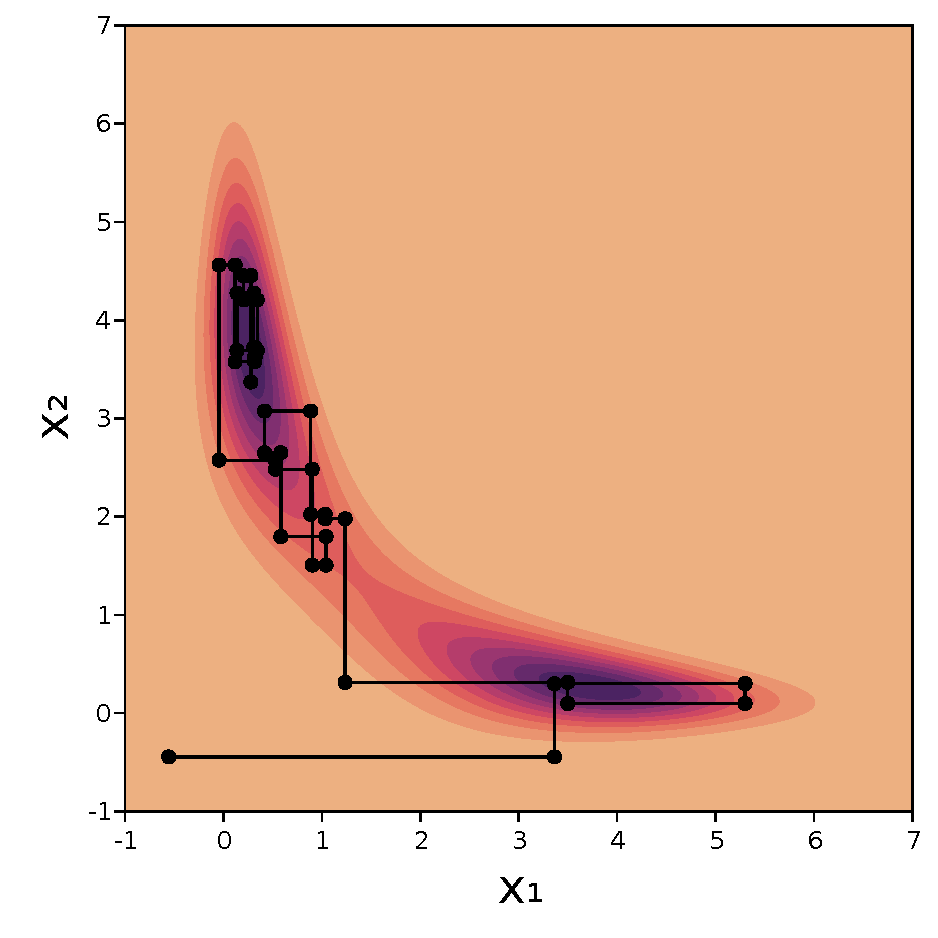
\includegraphics[width=0.5\textwidth]{./chapters/2_background/figures/gibbs_sampling.pdf}
\caption{20 steps of the Gibbs sampler trajectory on the Rosenbrock distribution in 2 dimensions.}
\label{fig:gibbs_samp}
\end{figure}

The Gibbs sampling approach is a conundrum.
On the one hand, sampling each component using the full-conditional is easy since it only involves drawing a scalar.
However, reforming a sampler for each full-conditional can be slow and costly.
The sampler can also get stuck or move very slowly if the components are highly correlated.
We can solve these drawbacks by using additional techniques like the \textbf{blocked Gibbs sampler} \cite{jensen1995blocking} where we sample groups of variables jointly, or \textbf{collapsed Gibbs sampling} \cite{liu1994collapsed} where we marginalize out some variables from the full-conditional distributions.
But blocked or collapsed updates are much less available and require heavier sampling machinery.

The augmentations proposed in this thesis allow using both the blocked and collapsed version by deriving the full-conditionals for each group of variables analytically.
Experiments show that the correlations between each group of variables are very low, and the sampler converges to the stationary distribution very fast.


\paragraph{Hamilton/Hybrid Monte Carlo}\mbox{}\\
\label{sec:hmc}
\acf{HMC} or Hybrid Monte Carlo \cite{duane1987hybrid, betancourt2017conceptual} is a \ac{MCMC} methods using Hamiltonian dynamics to make a new proposal.
We augment $\btheta^t$ with an extra momentum $\boldsymbol{p}^t$ sampled randomly for every proposal from $\No(0,M)$ where $M$ is the mass matrix.
Next we run the Hamiltonian dynamics based on the Hamiltonian $H(\btheta, \boldsymbol{p}) = -\log \pi(\btheta) + \frac{1}{2}\boldsymbol{p}^\top M \boldsymbol{p}$ over $L$ leapfrog steps with step size $\Delta t$.
The proposal at time $L\Delta t$ is accepted or rejected based on the acceptance rate:
\begin{align*}
    A = \min\left(1, \frac{\exp(-H(\btheta(L\Delta t), \boldsymbol{p}(L\Delta t)))}{\exp(-H(\btheta(0), \boldsymbol{p}(0)))}\right)
\end{align*}
The Hamiltonian is normally perfectly conserved when using a symplectic integrator like the leapfrog algorithm.
We get high acceptance rates while the dynamics lower the correlation between each sample by exploring the parameter space more freely than a basic random walk.
We give an illustration of the process in Figure~\ref{fig:hmc}, where we draw the Hamiltonian dynamics path with gray lines.

The \ac{HMC} algorithm requires the tuning of its parameters $M$, $L$, and $\Delta t$, which can be done by running 
A proper tuning of the algorithm guarantees the acceptance rate to be close to 1.


\ac{HMC} also has multiple disadvantages: 
First, one needs to integrate differential equations based on gradients, which becomes increasingly expensive for high-dimensional models and complex likelihoods.  \com{clarify better what is meant}
Second, it contains tunable parameters, namely the step size of the integrator, the number of steps taken, and the momentum parameters used.
These parameters can be locally optimized, but they are without guarantees and require additional computational time. \com{change the guarantee speech}
Last but not least, \ac{HMC} only works for continuous variables.

\begin{figure}[H]
    \centering
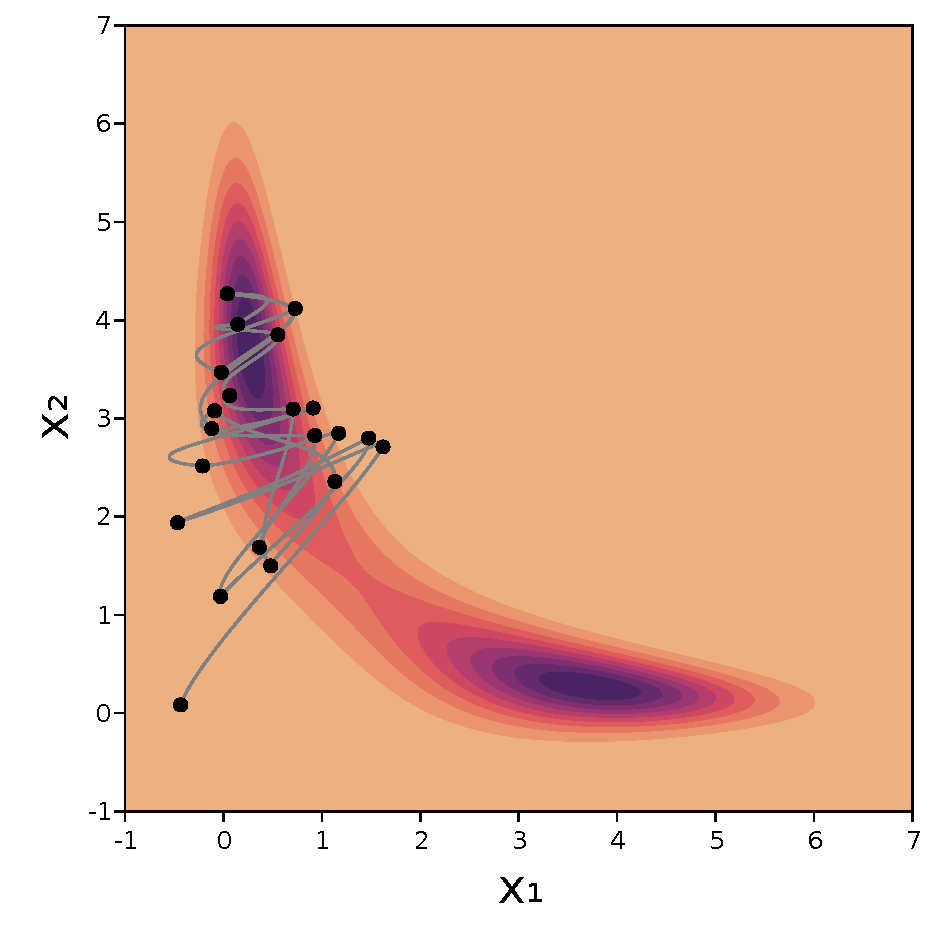
\includegraphics[width=0.5\textwidth]{./chapters/2_background/figures/hmc_sampling.pdf}
\caption{Illustration of the HMC sampler (gray lines are the Hamiltonian dynamics)}
\label{fig:hmc}
\end{figure}


\paragraph{The choice of sampler}\mbox{}\\
There are other strong choices such as elliptical slice sampling \citet{murray2010elliptical} which are particularly well-fitted for Gaussian priors.

The choice of the sampling algorithm is a complex one and is extremely problem-dependent.
\ac{HMC} is more of a jack-of-all-trades which has its plug-and-play practicality, in particular in regard to recent advances in automatic differentiation which removed the requirement to compute gradients by hand.
Gibbs sampling has the disadvantage of requiring upstream work and to only work in specific situations.
Nonetheless, it proved to be an algorithm of choice in the different works presented in this thesis.

\subsection{Variational Inference}
\label{sec:vi}
\acf{VI}, also called Variational Bayes, consists in approximating the posterior $p(\btheta|\bX)$ with another distribution $q(\btheta)$.
Given a family of distributions $\mathcal{Q}$, parametrized by the variational parameters $\bphi$, one aims to solve the following optimization problem:
\begin{align}
\bphi^* = \arg_{\bphi}\min \mathcal{D}\left(q_{\bphi}(\btheta), p(\btheta|\bx)\right),
\label{eq:prob_VI}
\end{align}
where $\mathcal{D}$ is a distance between two distributions and $q_{\bphi}$ is the distribution $q\in \mathcal{Q}$ parametrized by $\bphi$.
One of the most used dissimilarity measure is the backward \ac{KL} divergence, defined for continuous distributions as:
\begin{align}
\KL{q(x)}{p(x)} = \int q(x) \log \frac{q(x)}{p(x)}dx
\label{eq:kl}
\end{align}

The objective of Equation~\eqref{eq:prob_VI} or \eqref{eq:kl} is generally not directly tractable when the normalizer is not known.
Since $p(\btheta|\bx)$ involves the normalization constant $p(\bx)$, one resorts to a surrogate function, the \ac{VFE} (or its negative counterpart the \ac{ELBO}):
\begin{align}
\KL{q_{\bphi}(\btheta)}{p(\btheta|\bx)} =& \int q_{\bphi}(\btheta) \left(\log q_{\bphi}(\btheta) - \log p(\btheta|\bx)\right)d\btheta\\
=&\int q_{\bphi}(\btheta) \left(\log q_{\bphi}(\btheta) - \log p(\btheta, \bx) - \log p(\bx)\right)d\btheta\\
=&\underbrace{- \log p(\bx)}_{:=C} + \int q_{\bphi}(\btheta) \left(\log q_{\bphi}(\btheta) - \log p(\bx|\btheta)- \log p(\btheta) \right)d\btheta\\
=& C -\expec{q_{\bphi}}{\log p(\bx|\theta)} + \KL{q_{\bphi}(\btheta)}{p(\btheta)} = \VFE(\bphi) + C
\end{align}


By minimizing the \ac{VFE}, $\VFE(\bphi)$, instead of the \ac{KL} divergence, we can expect to find a solution close to the optimum of the problem stated in \eqref{eq:prob_VI}.\com{fix comment on minimizing}

A standard way to find the $\bphi^* = \arg\min \VFE(\bphi)$ is to perform gradient descent on the variational parameters $\bphi$:
\begin{align}
\bphi^{t+1} = \bphi^{t} - \epsilon \grad_{\bphi}\VFE(\bphi^{t}).
\label{eq:vigraddescent}
\end{align}

Computing the gradient $\grad_{\bphi}\VFE(\bphi)$ can be non-trivial, as it involves derivatives over expectations, but tricks like reparametrization \cite{titsiasDoublyStochasticVariational} help reducing the cost of these computations.

The choice of the family $\mathcal{Q}$ is a trade-off decision.
A richer, more complex family will probably be able to approximate the posterior better but computing the \ac{KL} and optimizing the variational parameters will be increasingly difficult.
A standard example is the \ac{VGA}\footnote{The \ac{VGA} is explored in more details in Chapter~\ref{ch:gpf}.}, where the variational distribution $q_{\bphi}$ is a Gaussian, i.e. $\mathcal{Q} = \left\{q \sim \mathcal{N}(\boldm, S)\right\}$, and $\bphi = \{\boldm, S\}$.
One can decide to restrict $\mathcal{Q}$ further by specifying the structure of $S$.
Forcing it to be diagonal will simplify a lot of computations and avoid inverse matrix operations, but all variable dependencies are lost.
This is what the mean-field approximation is about.

\paragraph{Mean-Field Approximation}\mbox{}\\
One problem when considering $q_{\bphi}(\btheta)$ is that if we consider that all parameters are correlated to each other, the number of variational parameters to train grow quadratically with the dimensionality of $\btheta$.
The simplest assumption is the \ac{MF} approximation. \com{reformulate}
The \ac{MF} assumption is that every component of $\btheta$ to be independent of each other.
This variational family can be specified as:
\begin{align}
    \mathcal{Q}_{MF}= \left\{q = \prod_{i=1}^D q_{\bphi_i}(\theta_i)\right\},
\end{align}
where $\bphi_i$ are the variational parameters for the variable $\theta_i$.

One can also build more general distributions by considering independence between blocks of variables instead.
Given $\mathcal{I}=\{1,2,\ldots,D\}$, the set of indices of $\theta$, we can build into $K$ independent subsets $\mathcal{I}_k \subseteq \mathcal{I}$ such that  $\mathcal{I} = \cup_{k=1}^K \mathcal{I}_{k}$ and $\mathcal{I}_i \cap \mathcal{I}_j=\emptyset,~\mathrm{iff}~i \neq j$.
The variational distribution based on this \ac{BMF} approximation is then defined as
\begin{align}
    q^{BMF}_{\bphi}(\btheta) = \prod_{k=1}^K q_{\bphi_k}(\btheta_{\mathcal{I}_k}),
\end{align}
where $\bphi_k$ are the variational parameters for the set of variable $\btheta_{\mathcal{I}_k}$.

\paragraph{Coordinate Ascent VI}\mbox{}\\
\label{sec:cavi}
Based on the \ac{MF} and \ac{BMF} approach, we are interested in finding the solution for each set of parameters $\bphi_i$ to
\begin{align}
    \bphi_i^* = \arg_{\bphi_i}\min \VFE(\bphi_i, \bphi_{/i}),
    \label{eq:optimalbphi}
\end{align}
i.e. by keeping all other parameters fixed, what is the optimal $\bphi_i^*$.
This can be found either by solving
\begin{align}
\left.\grad_{\varphi_i}\VFE(\bphi)\right\vert_{\varphi_i=\varphi_i^*} = 0,
\end{align}
or performing the same gradient scheme as Equation~\eqref{eq:vigraddescent}.
The solution to Equation~\eqref{eq:optimalbphi} is given by
\begin{align}
q_{\bphi_i}^*(\btheta_i) \propto \exp\left(\expec{q_{\bphi}(\btheta_{/i})}{\log p\left(\btheta_i|\btheta_{/i},\bx\right)}\right)
\end{align}
where $\btheta_{/i}$ represent the collection of variables $\btheta_{/i} = \{\theta_j | j \neq i\}$.\com{mention only normalizable sometimes}
The distribution $p(\btheta_i|\btheta_{/i},\bx)$ is the full-conditional distribution as described in Section~\ref{sec:posterior}.

When working with distribution coming from exponential families, it is straightforward to get the optimal variational parameters $\bphi$.
By updating the parameters one after another we get a \ac{CAVI} scheme\footnote{The word ascent is used since the scheme was originally derived using the negative \ac{VFE} i.e. the \ac{ELBO}.}.
Effectively, one updates each variational parameter $\bphi_i$ with its optimum given the rest of the variational parameters $\bphi_{/i}$ via closed-form functions:
\begin{align}
\varphi_i^{t+1} = f_i\left(\bphi_{1:(i-1)}^{t+1}, \bphi_{(i+1):D}^t\right).
\end{align}
\com{define f}
The order of the updates does not matter as long as the variational parameters $\bphi$ are initialized in their domain.
Note also that, similarly to the Gibbs sampling algorithm, inference can be made further by proceeding to \textbf{block updates}, working with set of variables instead one at a time.

The full algorithm is presented on Algorithm~\ref{alg:CAVI}.

\begin{algorithm}
    \caption{\ac{CAVI} Updates}
    \label{alg:CAVI}
    \begin{algorithmic}
        \While {$|\VFE^{t+1} - \VFE^t| > \epsilon$}
            \ForAll {$i \in \{1,\ldots,D\}$}
                \State $\bphi_i^{t+1} = f_i\left(\bphi_{1:(i-1)}^{t+1}, \bphi_{(i+1):D}^t\right).$
            \EndFor
        \EndWhile
    \end{algorithmic}
\end{algorithm}


\paragraph{Natural Gradients}

One interesting aspect of \ac{CAVI}, is that it implicitly uses \textbf{natural gradients} \cite{amariNaturalGradientWorks1998}.
A natural gradient is a gradient preconditioned with the inverse Fisher information matrix defined as
\begin{align}
    \mathcal{I}_\theta = \expec{p(\bx|\btheta)}{\left(\grad_{\btheta}\log p(\bx|\btheta)\right)\left(\grad_{\btheta} \log p(\bx|\btheta)\right)^\top} = -\expec{p(\bx|\btheta)}{\mathbf{H}(\log p(\bx|\btheta))},
    \label{eq:fisherinfomatrix}
\end{align}
where $\mathbf{H}(f)$ is the Hessian matrix of the function $f$.
The Fisher information matrix is a Riemannian metric which gives the direction of the steepest descent with respect to the KL divergence.
\com{Give more details about the meaning of the Fisher info}
The natural gradient is given by :
\begin{align*}
    \widetilde{\grad}_{\bphi}\mathcal{F}(\bphi) = \mathcal{I}^{-1} \grad_{\bphi}\mathcal{F}(\bphi)
\end{align*}
The natural gradient is constructed such that the metric it gives maximizes the change of the infinitesimal \ac{KL} divergence between the given distribution and its target.
The reason why natural gradients are brought up here is that the updates of the \ac{CAVI} algorithm \ref{alg:CAVI} for exponential distributions, can be interpreted as natural gradient ascent updates with learning rate $1$.
\begin{align*}
    \bphi^{t+1} = \bphi^t + \mathcal{I}^{-1}_\theta\grad_{\bphi}\mathcal{F}(\bphi^t) \equiv \bphi^{t+1}
\end{align*}
\com{maybe be more explicit about this}

\subsection{Scale-Mixtures and conditionally conjugate likelihoods}
\label{sec:scale-mixtures}
A large part of this work is based on scale-mixtures and mixtures in general.
A scale-mixture is a continuous mixture of a distribution with a varying scale parameter.
A textbook example is the Student-T distribution which is a Gaussian scale-mixture with a Gamma distribution on the scale weights:
\begin{align*}
    T_\nu(x) = \int_{0}^\infty \mathcal{N}\left(x|0,\omega\right)\mathrm{Ga}\left(\omega|\frac{\nu}{2}, \frac{\nu}{2}\right)d\omega,
\end{align*}
where $\mathrm{Ga}$ is a Gamma distribution.
Another example is the Laplace distribution which is also a Gaussian scale-mixture:
\begin{align*}
    \mathrm{La}(x|\beta) = \int_0^{\infty} \mathcal{N}(x|0,\omega)\mathrm{Exp}\left(\omega|\frac{1}{2b^2}\right)d\omega,
\end{align*}
where $\mathrm{Exp}$ is the exponential distribution.

Generally these representations appear in the computation of predictive distributions.
For example in linear regression with a Gamma prior on the likelihood variance, the resulting posterior predictive distribution will be a Student-T distribution.
In this thesis we show that we can use this connection the other way around.
Given a likelihood $p(\bx|\btheta)$ which can be defined as a marginalized scale-mixture,
we can \textbf{augment} the likelihood by "unmarginalizing" the scale-mixture.
We transform for example a Student-T likelihood into a Gaussian likelihood with a Gamma prior.
This allows for so-called conditionally conjugate likelihoods.


Now that all important and necessary topics for this thesis have been overviewed, the following will present the different works presented in this thesis. 
% ---------------------------------------------------------------------------
% ----------------------- end of thesis sub-document ------------------------
% ---------------------------------------------------------------------------